\documentclass[tikz,border=10pt]{standalone}
\usepackage{tikz}
\begin{document}
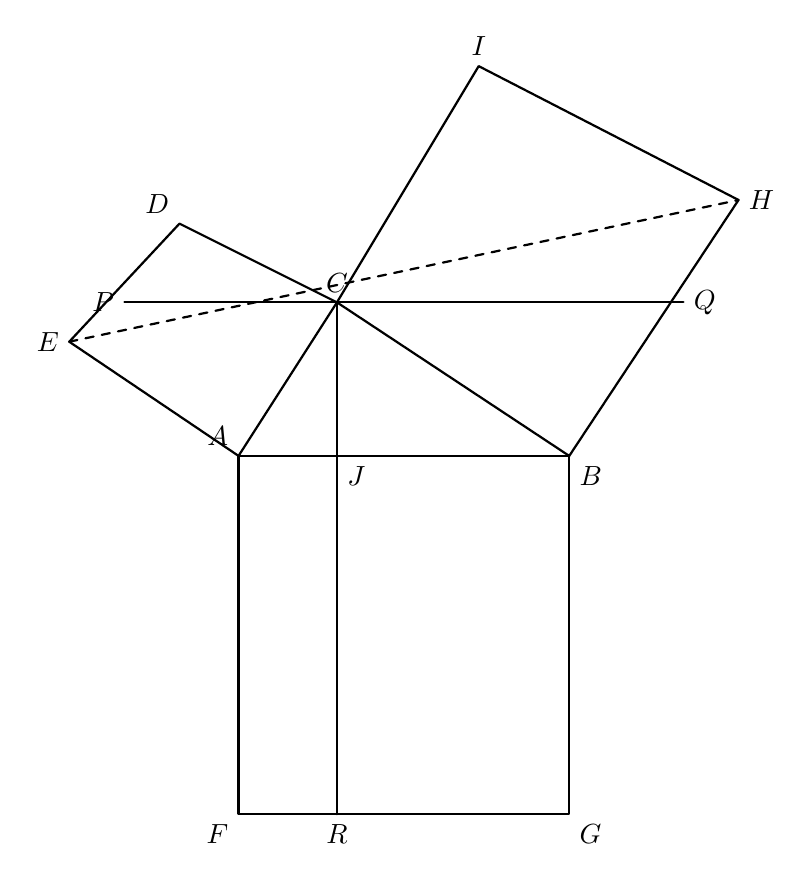
\begin{tikzpicture}[line cap=round,line join=round,thick]

% Coordinates
\coordinate (A) at (0,0);
\coordinate (B) at (4.2,0);
\coordinate (C) at (1.25,1.95);
\coordinate (D) at (-0.75,2.95);
\coordinate (E) at (-2.15,1.45);
\coordinate (P) at (-1.45,1.95);
\coordinate (I) at (3.05,4.95);
\coordinate (H) at (6.35,3.25);
\coordinate (Q) at (5.65,1.95);
\coordinate (J) at (1.25,0);
\coordinate (F) at (0,-4.55);
\coordinate (G) at (4.2,-4.55);
\coordinate (R) at (1.25,-4.55);

% Outer shapes
\draw (A)--(B)--(G)--(F)--cycle;
\draw (A)--(C)--(B);
\draw (A)--(E)--(D)--(C);
\draw (C)--(I)--(H)--(B);

% Interior and auxiliary lines
\draw (P)--(Q);
\draw (C)--(R);
\draw[dashed] (E)--(H);

% Labels
\node[above left] at (A) {$A$};
\node[below right] at (B) {$B$};
\node[above] at (C) {$C$};
\node[above left] at (D) {$D$};
\node[left] at (E) {$E$};
\node[left] at (P) {$P$};
\node[above] at (I) {$I$};
\node[right] at (H) {$H$};
\node[right] at (Q) {$Q$};
\node[below right] at (J) {$J$};
\node[below left] at (F) {$F$};
\node[below right] at (G) {$G$};
\node[below] at (R) {$R$};

\end{tikzpicture}
\end{document}
